\section{The Raft consensus algorithm}

Raft was proposed by Diego Ongaro and John Ousterhout in 2014. The goal was to offer a easy to understand, implementable and fault-tolerant consensus protocol to be used in a distributed system to replicate state machines. Raft works by managing a replicated log across multiple nodes and upholds simplicity by separating key elements of the process, that is leader election, log distribution and safety, versus a protocol like Paxos that has proven difficult to understand. Key features of Raft include:

\noindent \textbf{Strong leader:} The replication of log entries flow from the leader only. This simplifies log management, and enhances the leader role in Raft compared to other consensus protocols.

\noindent \textbf{Leader election:} From the start of the algorithm a leader has to be elected. Raft uses a randomized timer on each node to elect a leader. This is done to avoid conflicts and assumes all nodes are equally capable of being leaders. The time period electing a leader is called a term, and a new leader must be elected, if the old one fail.

\noindent \textbf{Membership changes:} Raft offers a join and leave command to dynamically change the membership of nodes. This is facilited by what is called a \textit{joint consensus} mechanism, that allows two different configurations to overlap while the transition is ongoing.

\noindent \textbf{Log replication:} The leader is responsible for replicating a log containing state information. During a term, client nodes (followers) send commands to the leader, and these are saved in a log. Upon replication, followers append the entries received from the leader in their own log. When a majority of followers have received the log, a leader adds it to his own state machine and it is then considered committed.

\noindent \textbf{Safety:} Only one leader can be elected for a given term. To ensure consistency, if a server has applied one log entry for an index in its log, then no other server can may apply a different value for the same index. Only a server with the newest log can become leader.

\noindent We will now look at the fundamentals for the protocol. We assume a cluster of five nodes ($N_1$ to $N_5$) participating in our Raft consensus algorithm. All nodes have a randomized timer $T_i$ = (i=1,2...,N).

\begin{figure}[H]
	\centering
	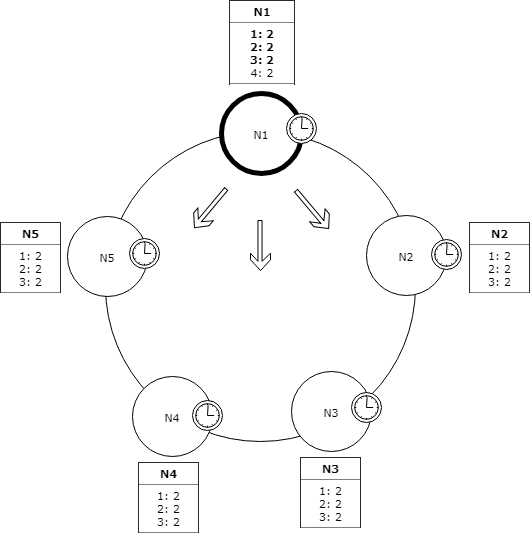
\includegraphics[scale=0.5]{faultTolerance/fig/Raft.png}
	\caption{The topology for our Raft setup. N1 is leader and replicates its state log to follower nodes.}
	\label{fig:raft}
\end{figure}


